
\section{Processi di supporto}\label{PS}

	\subsection{Documentazione}\label{PS:Documentazione}

		\subsubsection{Implementazione}\label{PS:Documentazione:Implementazione}

			\paragraph{Template}\label{PS:Documentazione:Implementazione:Template}
			Prima di iniziare a redigere i documenti, abbiamo creato un \gloss{template} per \LaTeX \ (\S\ref{LaTeX}) contenente tutte le impostazioni grafiche
			condivise tra questi, per sfruttare il riutilizzo del codice e semplificare enormemente la manutenzione dei sorgenti.\par
			Nello specifico, è presente un file per ognuna delle seguenti utilità:
			\begin{itemize}
				\item \gloss{Layout} delle pagine
				\item \gloss{Macro} personalizzate volte a semplificare l'utilizzo di strutture o comandi ricorrenti
				\item Codice per la generazione della prima pagina
					(struttura definita in \S\ref{PS:Documentazione:Struttura:Frontespizio})
				\item Diario delle modifiche
			\end{itemize}

			\paragraph{Ciclo di vita dei documenti}\label{PS:Documentazione:Implementazione:CicloVita}
			Durante il suo ciclo di vita, ogni documento potrà trovarsi in una delle seguenti fasi:
			\begin{itemize}
				\item \textbf{Redazione}: fase che inizia con la creazione del documento e dura fino alla sua ultima approvazione.
					Il \Res\ assegna ai \gloss{redattori} le varie sezioni di ogni documento da redigere, i quali aggiorneranno la versione nel diario delle modifiche
					come normato in \S\ref{Versionamento}.
				\item \textbf{Verifica}: il documento entra in questa fase nel momento in cui i Redattori hanno terminato la stesura del lavoro loro assegnato, segnalandolo al \Res, che a sua volta assegnerà ai Verificatori la verifica della qualità del prodotto, secondo quanto riportato nelle norme di verifica. Essi potranno approvare il documento oppure notificare il \Res\ su eventuali errori o incongruenze emerse durante la fase di verifica, che provvederà a riassegnare il lavoro.
				\item \textbf{Approvazione}: fase che inizia dall'accettazione del documento da parte dei Verificatori nella fase di verifica. Spetta al \Res\
					l'approvazione ufficiale del documento, seguita dal rilascio di una \gloss{major release}.
			\end{itemize}

		\subsubsection{Struttura}\label{PS:Documentazione:Struttura}

			\paragraph{Frontespizio}\label{PS:Documentazione:Struttura:Frontespizio}
			La prima pagina di ogni documento, sarà caratterizzata da:
			\begin{itemize}
				\item Logo e nome del gruppo
				\item Titolo del documento
				\item Informazioni sul documento:
					\begin{itemize}
						\item Versione documento
						\item Data di creazione e ultima modifica
						\item Nominativo dei Redattori
						\item Nominativo dei Verificatori
						\item Nominativo del \Res
						\item Destinazione d'uso
						\item Destinatari del documento
						\item Contatto del gruppo
					\end{itemize}
				\item Breve descrizione del documento
			\end{itemize}

			\paragraph{Storico delle versioni}\label{PS:Documentazione:Struttura:StoricoVersioni}
			La pagina che segue il frontespizio contiene lo storico delle versioni del documento, in cui ogni aggiunta o modifica significativa ha
			comportato un incremento di versione. Ogni riga contiene, a partire da sinistra:
			\begin{itemize}
				\item Il numero della versione nel formato espresso in \S\ref{Versionamento}
				\item Una breve descrizione delle modifiche apportate
				\item Il ruolo dell'autore che ha apportato la modifica
				\item Il nominativo dell'autore
				\item La data di modifica
			\end{itemize}
			La chiave primaria della tabella è il numero di versione ordinata in senso decrescente, in modo che la versione più vecchia sia
			l'ultima riga della tabella.

			\paragraph{Indice}\label{PS:Documentazione:Struttura:Indice}
			In ogni documento, esclusi i verbali, è presente un indice contenente tutte le sezioni, sottosezioni e paragrafi. I numeri di sezioni, sottosezioni,
			e paragrafi sottostanti saranno separati da un punto (e.g. 1.4.1).\par
			Saranno eventualmente presenti un indice delle
			figure e un indice delle tabelle, assenti in caso non ci siano tabelle o figure nel documento.\par
			I valori degli indici partono da 1.

			\paragraph{Contenuto}\label{PS:Documentazione:Struttura:Contenuto}
			La struttura di ogni pagina presenta:
			\begin{itemize}
				\item Intestazione con:
				\begin{itemize}
					\item A sinistra, logo di \gruppo
					\item A destra, nome del capitolato e documento corrente
				\end{itemize}
				\item Piè di pagina con:
				\begin{itemize}
					\item A sinistra, nome e mail di riferimento del gruppo
					\item A destra, numero della pagina corrente
				\end{itemize}
			\end{itemize}


		\subsubsection{Design}\label{PS:Documentazione:Design}

			\paragraph{Norme tipografiche}\label{PS:Documentazione:Design:NormeT}
			Le norme tipografiche qui di seguito elencate sono state decise in modo che ognuno di noi concorra a mantenere una forma coerente e univoca
			per tutti i documenti redatti.

			\subparagraph{Stile redazionale}
			Lo stile redazionale dei vari documenti sarà prevalentemente personale, in prima persona, per rendere chiaro il soggetto delle frasi.

			\subparagraph{Stile del testo}\label{PS:Documentazione:Design:NormeT:StileTesto}
			\begin{itemize}
				\item \textbf{Corsivo}: solo per i nomi dei documenti citati.
				\item \textbf{Maiuscolo}: la prima lettera per
				\begin{itemize}
					\item Tutte le parole appartenenti ai nomi dei documenti tranne gli articoli
					\item Nomi dei ruoli
					\item Prima parola degli elenchi puntati
				\end{itemize}
			\end{itemize}

			\subparagraph{Elenchi puntati}\label{PS:Documentazione:Design:NormeT:ElenchiPuntati}
			\begin{itemize}
				\item \textbf{Simboli di livello}: un pallino nero per il primo livello, un trattino per il secondo livello.
				\item \textbf{Punteggiatura}: nessuna punteggiatura alla fine di una frase, tranne nel caso in cui sia presente una descrizione.
					In quel caso la descrizione è preceduta dai due punti ``:'' e termina con un punto ``.''.
				\item \textbf{Grassetto}: solo se è presente una descrizione, allora sono in grassetto tutte le parole prima dei due punti ``:''.
			\end{itemize}

			\subparagraph{Altri formati testuali comuni} \label{PS:Documentazione:Design:NormeT:AltriFormati}
			\begin{itemize}
				\item \textbf{Orari}: \texttt{HH:MM} secondo la norma ISO 8601\footnote{Riferirsi alla voce
				%``ISO 8601''
				1
				in \S\ref{rifinfo}}
				nel formato 24 ore dove:
				\begin{itemize}
					\item \texttt{HH} indica le ore, da 00 a 23
					\item \texttt{MM} i minuti, da 00 a 59
				\end{itemize}
				\item \textbf{Date}: \texttt{YYYY-MM-DD} formato adottato in Europa dove:
				\begin{itemize}
					\item \texttt{YYYY} l'anno
					\item \texttt{MM} il mese, da 01 a 12
					\item \texttt{DD} il numero del giorno, da 01 a 31
				\end{itemize}
				\item \textbf{Nota a piè di pagina}: serve ad inserire elementi aggiuntivi, come osservazioni o riferimenti a parti interne al documento, utili alla comprensione del testo,
				ma se inseriti all'interno del discorso, ne interromperebbero la lettura, rendendola meno scorrevole.
			\end{itemize}


			\paragraph{Elementi grafici}

			\subparagraph{Figure}
			Ogni immagine inserita nei documenti deve sempre essere centrata rispetto al foglio e adeguatamente separata dal testo. Deve inoltre essere
			accompagnata da una breve \gloss{caption} che permetta al lettore di capire esattamente che cosa sta guardando.\\
			È presente nell'indice l'elenco delle figure che raccoglie la lista di tutte le immagini presenti.

			\subparagraph{Tabelle}\label{StrumentiDiSupportoTabelle}
			Come per le figure, ogni tabella sarà accompagnata da una caption e sarà della dimensione del testo, o se più piccola, centrata.
			Tutte le tabelle saranno raccolte nell'elenco delle tabelle.\par
			Saranno presenti due tipologie di tabelle:
			\begin{itemize}
				\item \textbf{Semplici}: tabelle standard senza uno stile particolare, in cui le celle sono separate da bordi neri (evitare, ove non risulta necessario,
					le righe verticali).
				\item \textbf{Complesse}: tabelle con un'alternanza di colori tra le righe delle celle (grigio e bianco) e senza bordi verticali.
					Le celle sono separate orizzontalmente da una corretta spaziatura e allineamento e verticalmente dall'alternanza dei due colori.
					La riga dell'\gloss{header} può essere bianca o di un grigio più scuro in base al contesto, con il testo che può essere in grassetto.
			\end{itemize}

			% 6.1.2.3 The prepared documents shall be reviewed and edited for format, techni cal content, and presentation style agai nst their documentation standards. The y shall be approved for ade quacy by authorized personnel prior to issue.
			\paragraph{Approvazione}	\label{Approvazione}
			Ogni documento, nel momento in cui viene ritenuto pronto, deve essere revisionato dal \Res\ affinché ne venga controllata l'adeguatezza e approvato il rilascio.


		\subsubsection{Produzione}

			\paragraph{Suddivisione dei documenti}\label{SuddivisioneDeiDocumenti}

			\subparagraph{Documenti interni}
			Le \NdPd\ e lo \SdFd\ sono documenti interni, consultabili solo dal team e dal committente, per motivi didattici.

			\subparagraph{Documenti esterni}
			Sono considerati esterni, invece, il \PdPd, il \PdQd, il \Gld\ e l'\AdRd\ che, al contrario dei precedenti, vengono consegnati al proponente.

			% Questi documenti sono ufficiali e approvati direttamente dal \Res\ e comprendono, per esempio: \PdP, \PdQ\ e \AdR. Si chiamano esterni perché accessibili al committente.

            \subparagraph{Verbali}\label{Verbali}
			Redigiamo questi documenti successivamente alle riunioni tenute	o in caso di incontri con \gloss{stakeholder} esterni, per esempio con \II. Una singola persona ha il compito di stendere
			la relazione relativa al verbale, presentando le seguenti sezioni:
			\begin{itemize}
				\item \textbf{Informazioni incontro}: lista delle informazioni principali riguardanti la riunione quali luogo, data, orario, ordine del giorno, ecc.
				\item \textbf{Argomenti}: lista dei principali argomenti trattati, con breve descrizione.
				\item \textbf{Tracciamento delle decisioni}: contiene il resoconto delle decisioni prese nella riunione, tracciate con un codice nel formato \texttt{yyyy-mm-dd-n}, dove \texttt{yyyy-mm-dd} è
				la data in cui si è tenuta la riunione e \texttt{n} è il numero della decisione presa, che parte da 1.

			\end{itemize}


			\paragraph{Strumenti di supporto}\label{StrumentiDiSupporto}

			\subparagraph{\LaTeX}\label{LaTeX}
			Per la stesura della documentazione abbiamo deciso di utilizzare il linguaggio di \gloss{markup} \LaTeX\ perché presenta molti vantaggi, tra i quali:
			\begin{itemize}
				\item Supporta nativamente il \gloss{versionamento}, essendo un linguaggio compilato
				\item Supporta la modularità, rendendo più facile organizzare un documento dividendone logicamente i vari moduli
				\item Permette il riutilizzo del codice tramite l'uso di macro già pronte o personalizzate, oppure includendo lo stesso \gloss{sorgente} in punti diversi
				\item Gestisce automaticamente indici e riferimenti
			\end{itemize}

			\subparagraph{Google Drive}\label{GoogleDrive}
			Per la condivisione di file informali, tabelle informative e diagrammi dei casi d'uso e delle classi (con \hyperref[drawio]{draw.io}), utilizziamo lo strumento
			di cloud Google Drive. Esso ci permette di tenere file informativi sempre aggiornati e condivisi tra tutti i membri del team, raggiungibili in qualunque momento
			anche da smartphone. Altre informazioni sono reperibili tramite i link informativi in \S\ref{rifinfo}.

			\subparagraph{TexStudio/Visual Studio Code}
			TexStudio e Visual Studio Code sono i due ambienti di sviluppo scelti per stilare la documentazione.
			TexStudio è un \gloss{IDE} nativo per l'utilizzo di \LaTeX. Visual Studio Code è un editor intelligente moderno (alla pari di un \gloss{IDE}) che, tramite
			estensioni, permette il supporto di praticamente ogni linguaggio.
			Entrambi permettono una rapida compilazione e un'istantanea visualizzazione dell'anteprima del PDF prodotto, oltre agli altri vantaggi che ogni IDE offre,
			tra cui: suggerimenti e completamenti automatici delle parole chiave, ricerca intelligente (eventualmente tramite \gloss{regexp}) controllo ortografico della
			lingua italiana o inglese e così via.\\
			Più informazioni sono reperibili sui rispettivi siti ufficiali, i cui link sono presenti in \S\ref{rifinfo}.
			% \subparagraph{Visual Studio Code}

			\subparagraph{GanttProject}
			GanttProject è un programma gratuito dedicato alla formazione dei diagrammi di Gantt. Permette di creare task e milestone, organizzare le task in lavoro
			strutturato a interruzioni, disegnare i vincoli di dipendenza tra di esse e molte altre utilità, generando automaticamente il relativo diagramma.
			Per maggiori informazioni, si rimanda alla fonte ufficiale (consultare \S\ref{rifinfo}).

			\subparagraph{Draw.io}\label{drawio}
			Draw.io è un'applicazione web in grado di creare diagrammi UML, di Entità-Relazionale, di flusso e molto altro. Il motivo che ci ha portato
			a scegliere questo strumento è la sua perfetta integrazione con \gloss{Google Drive}, oltre al suo alto livello di intuitività.
			Questo permette la condivisione dei diagrammi creati tra tutti i collaboratori in ogni momento e in modo automatico.
			Per maggiori informazioni, visualizzare la fonte ufficiale (\S\ref{rifinfo}).

			\subparagraph{Indice di Gulpease}
			Si tratta di un indice di leggibilità dei documenti in lingua italiana. A differenza degli indici per le altre lingue, questo si basa sulla lunghezza delle parole in lettere e non in sillabe. In base al valore indicato si può capire che livello di istruzione deve possedere una persona per comprendere il documento.\\
            Per automatizzare il calcolo di questo indice è stato prodotto uno \gloss{script} che viene eseguito ad ogni \gloss{commit} nella \gloss{repository}, il quale riporta in un file i risultati ottenuti. Tale indice è descritto anche in \S\ref{AnalisiStatica:Gulpease}.

			\subparagraph{Controllo ortografico}
			Per il controllo ortografico utilizziamo:
			\begin{itemize}
				\item In fase di redazione dei documenti, il controllo ortografico integrato degli IDE utilizzati
				\item In fase di verifica, lo strumento GNU Aspell, uno strumento open source per il controllo ortografico che permette tramite interfaccia interattiva di cambiare parole non riconosciute dal dizionario e scegliere tra più suggerimenti. Maggiori informazioni alla fonte ufficiale, reperibile in \S\ref{rifinfo}.
				La correttezza ortografica possiede una metrica presente in \S\ref{AnalisiStatica:CorrettezzaOrtografica}.
			\end{itemize}

            \subparagraph{Glossarizzazione dei ternimi}
			Come spiegato in \S\ref{GlossarioDocumentiEsterni}, i termini con un particolare significato vengono riportati e definiti all'interno di \Gld. Per automatizzare questo processo è stato creato uno script che valuta le voci all'interno di \Gld\ e ed inserisce i riferimenti a queste voci alla prima occorrenza di ogni parola in tutti i documenti prodotti.

			% 6.1.3.2 Controls shall be established in accordance with the Configuration Management Process (6.2).
			\paragraph{Controllo}	\label{Controllo}
			I controlli devono essere stabiliti in concordanza con il processo di configurazione alla sezione \S\ref{Configurazione}.

			% Da Breaking Bug
			\subparagraph{Controllo sui processi}	\label{ControlloProcessi}
			Per il controllo della qualità sui processi abbiamo scelto di seguire in ordine tre attività principali:
			\begin{enumerate}
				\item \textbf{Misurazione}: misurazione del processo al fine di accertarne la conformità con gli obiettivi.
				\item \textbf{Analisi}: precisa analisi dei risultati e problemi rilevati nel processo.
				\item \textbf{Rettifica}: modifiche correttive volte alla risoluzione dei problemi che contribuiranno alla nuova misurazione del prossimo ciclo di procedure.
			\end{enumerate}
			Seguendo le attività passo per passo e ripetendo la sequenza più volte è possibile aiutarci a diminuire i costi di sviluppo in maniera considerevolmente vantaggiosa.
			% Al termine di ogni periodo viene valutato lo stato di avanzamento del progetto

			\subparagraph{Controllo sui prodotti}	\label{ControlloProdotti}
			Per le procedure di misurazione del prodotto effettuiamo:
			\begin{itemize}
				\item Uso delle metriche e delle procedure delineate nel documento corrente e dei test descritto nel \PdQd
				\item Confronto di tali risultati rispetto agli obiettivi prefissati \footnote{Consultabili nelle appendici del \PdQd}
				\item Valutazioni per il miglioramento \footnote{Consultabili anch'esse nelle appendici del \PdQd}
			\end{itemize}
			A questo scopo utilizziamo strumenti di analisi statica e dinamica presenti nella sezione \S\ref{Verifica}.


		\subsubsection{Mantenimento dei documenti}\label{Mantenimento}
		% 6.1.4.1 The tasks, that are required to be performed when documentation is to be modified, shall be
		% performed (see 5.5). For those documents that are under configuration mana gement, modifications
		% shall be mana ged in accordance with the Configu ration Mana gement Process (6.2).
		I documenti sotto l'attività di gestione delle configurazioni devono essere gestiti secondo il processo di configurazione alla sezione \S\ref{Configurazione}.

			\paragraph{Continuous Integration}\label{ContinuousIntegration}
			Per la produzione dei documenti adotteremo la pratica della \gloss{Continuous Integration}.
			Per questa attività il principio sarà limitato a sincronizzarsi il prima possibile con la repository remota (non essendoci una vera e propria build o dei test da effettuare),
			sia per quanto riguarda il \gloss{fetch} che per il \gloss{push}.
			Questo serve a rendere più remota possibile la probabilità di incappare nell'\gloss{Integration Hell}.

			\paragraph{Nomenclatura}

			\subparagraph{Verbali}	\label{NomenclaturaVerbali}
			I Verbali  possono essere interni oppure esterni, nel caso in cui il team incontri gli esponenti di \II\ o il committente.
			Il nominativo del file in cui sono formalizzati è il seguente:
			\begin{itemize}
				\item \texttt{VI\_yyyy-mm-dd.pdf} per i verbali interni
				\item \texttt{VE\_yyyy-mm-dd.pdf} per i verbali esterni
			\end{itemize}
			dove yyyy-mm-dd è la data in cui sono stati tenuti, nel formato descritto nel paragrafo \S\ref{PS:Documentazione:Design:NormeT:AltriFormati}. \par
            Al termine del documento è presente una tabella contenente il tracciamento delle decisioni prese durante l'incontro descritto nel verbale. Tali decisioni possiedono un identificativo definito:
            \begin{center}
                \texttt{[Nominativo file].[Numero progressivo]}
            \end{center}
            Ad esempio, VE\_2019-03-23.1.

			\subparagraph{Documenti vari}
			Saranno presenti due tipologie di file: file interni ad \gruppo\ e file esterni.
			\begin{itemize}
				\item La prima categoria include moduli di \LaTeX\ contenenti le varie sezioni e che non verranno mai esposti esternamente. Questi file verranno
					denominati usando la convenzione \texttt{snake\_case.tex}, dove snake\_case è il nome della sezione o modulo
				\item La seconda categoria include i file \texttt{.tex} principali che produrranno i PDF da consegnare al committente. Essi verranno denominati
				con la convenzione \mbox{\texttt{CamelCase vX.Y.Z.pdf}}, dove CamelCase sarà il nome del documento generico mentre \texttt{vX.Y.Z}
				sarà la versione che identifica univocamente il documento come descritto in \S\ref{Versionamento}
			\end{itemize}


	% \subsection{Codice sorgente}\label{PS:Codice}

		\subsubsection{Mantenimento del codice sorgente}\label{MantenimentoCodice}

			\paragraph{Continuous Integration}\label{CI}
			Anche per quanto riguarda il processo di codifica verrà adottato il principio di Continuous Integration.

			\subparagraph{Jenkins}\label{Jenkins}
			Per quanto concerne il codice sorgente usiamo il tool Jenkins per tenere sotto controllo la CI pipeline, definita come una deployment pipeline priva degli ultimi stadi relativi al deploy.\par
			Jenkins ci consente di amministrare in modo immediato tutti i passi dello sviluppo, nell'ordine:
			\begin{itemize}
				\item \textbf{SCM checkout}: sincronizzazione del codice con la repository remota.
				\item \textbf{Build}: build del codice su docker container.
				\item \textbf{Unit Test}: test di unità tramite Pytest\footnote{Riferirsi alla voce
				% ``Pytest''
				17
				in \S\ref{rifinfo}}.
				\item \textbf{Integration Test}: test di integrazione tramite Pytest.
				\item \textbf{System Test}: test per verificare il comportamento dell'intero sistema tramite \gloss{tox}.
			\end{itemize}

			Configuriamo Jenkins tramite Jenkinsfile e la CI pipeline viene eseguita in automatico, in modo da avere sempre sotto controllo la correttezza del codice sulla repository.

			\paragraph{Docker}\label{Docker} % TODO inserire immagine con i container attivi da Dockstation
			Per rendere il sistema Butterfly completamente isolato dal sistema circostante, creiamo dei container specifici per ogni componente. Per fare ciò, utilizziamo
			\gloss{Docker}\footnote{Riferirsi alla voce
			%``Docker''
			5
			in \S\ref{rifinfo}.},
			un tool che rende questo processo estremamente semplice. Sarà presente un'immagine Docker per ognuna delle seguenti componenti, dalle quali sarà possibile costruire un container:
			\begin{itemize}
				\item Producer Redmine
				\item Producer GitLab
				\item Gestore Personale
				\item Consumer Email
				\item Consumer Telegram
			\end{itemize}
			Attraverso l'uso di uno specifico \texttt{docker-compose.yml} e il comando \texttt{docker-compose up} il processo di build e avvio dell'applicativo sarà semplice e immediato.

			\subparagraph{DockerHub}\label{DockerHub}
			Per evitare di effettuare una build manuale dell'immagine di Docker contenente una specifica componente del software, abbiamo deciso di utilizzare DockerHub collegato alla nostra repository in GitHub. In questo modo ogni modifica effettuata nella repository, attraverso push sui branch master e develop, scatta una build automatica. Questa prevede quindi la creazione di dieci immagini salvate su cinque repository su DockerHub in un account denominato `alphasix'. Le immagini sono classificate in questo modo nome\_account/nome\_repository:tag:
			\begin{itemize}
				\item alphasix/producer-gitlab:master
				\item alphasix/producer-gitlab:develop
				\item alphasix/producer-redmine:master
				\item alphasix/producer-redmine:develop
				\item alphasix/gestore-personale:master
				\item alphasix/gestore-personale:develop
				\item alphasix/consumer-telegram:master
				\item alphasix/consumer-telegram:develop
				\item alphasix/consumer-email:master
				\item alphasix/consumer-email:develop
			\end{itemize}
			Il tag rappresenta il branch dal quale è stata effettuata la build.
			Le immagini con tag `master' saranno più stabili rispetto a quelle con altri tag, in quanto ancora in fase di sviluppo dato che possiedono funzionalità incomplete.


	\subsection{Configurazione}\label{Configurazione}

		% Tale e quale a 6.2 Configuration management process
		\subsubsection{Descrizione}	\label{Descrizione}
		Il processo di gestione delle configurazioni tratta di applicare procedure tecniche e amministrative attraverso il ciclo di vita del software per:
		\begin{itemize}
			\item Identificare, definire e fissare elementi software in un sistema
			\item Controllare modifiche e rilasci di questi elementi
			\item Registrare e fornire un resoconto del loro stato e delle richieste di modifica
			\item Assicurare la loro completezza, consistenza e correttezza
			\item Conrollare il loro immagazzinamento, gestione e consegna
		\end{itemize}
		Per questo motivo le attività che questo processo prevede sono:
		\begin{enumerate}
			\item Implementazione del processo
			\item Identificazione della configurazione
			\item Controllo della configurazione
			\item Resoconto dello stato della configurazione
			\item Valutazione della configurazione
			\item Gestione del rilascio e consegna
		\end{enumerate}
		Nello specifico, i sorgenti e i documenti ufficiali del gruppo vengono versionati utilizzando il sistema di controllo versione \gloss{Git}, strumento scelto vista la sua ampia diffusione e la sua integrazione con GitHub.
		La scelta di utilizzare un client grafico oppure i comandi da terminale è lasciata al singolo membro del team.

		%6.2.1.1 A configu ration mana gement plan shal l be develo ped . The plan shall describe: the configuration management activities; procedures and sched ule for performing these activities; the organ ization(s) responsible for performing these activities; and their rela tionship with other organ izations, such as software develop ment or maintenance. The plan shall be documented and imple mented.
		\subsubsection{Implementazione del processo}	\label{ImplementazioneProcesso}
		Ognuno di noi si deve attenere alle norme descritte nei prossimi paragrafi al fine di garantire l'identificazione di ogni versione dei prodotti.
		Ogni persona è responsabile di queste attività.
		L'\Amm\ si occupa di controllare versioni e configurazioni del prodotto.


		\subsubsection{Identificazione della configurazione} \label{IdentificazioneConfigurazione}
		Questa sezione determina le modalità con cui identifichiamo le versioni di ogni componente software e di ogni documento.

		\paragraph{Versionamento} \label{Versionamento}
		Tutti i documenti redatti, i file sorgente e il codice sorgente supportano il versionamento, in modo da essere univoci e rendere disponibile la possibilità di consultare versioni precedenti in qualsiasi punto del loro \gloss{ciclo di vita}.
		Il modello di versionamento adottato segue lo schema \gloss{change significance}.\par
		La versione di un file è espressa secondo la notazione
			\begin{center}
			\texttt{X.Y.Z}
			\end{center}
			\indent dove:
			\begin{itemize}
				\item \texttt{X} indica il numero di versione principale. Inizia da 0 e viene incrementato ogni volta che il \Res\ approva il documento o il sorgente in esame,
					determinando una major release
				\item \texttt{Y} indica il numero di versione secondario, contatore delle fasi di verifica effettuate dal \Ver\ superate positivamente.
					Inizia da 0. Viene azzerato ad ogni incremento della \texttt{X}
				\item \texttt{Z} è l'indice di modifica minore, incrementato ogni volta che viene effettuato un aggiornamento inferiore.
				Viene azzerato ad ogni incremento della \texttt{Y} o della \texttt{X}
			\end{itemize}

		\subsubsection{Resoconto dello stato della configurazione e struttura delle repository} \label{ResocontoConfigurazione}
		Una repository, essendo GitHub un \gloss{version control system}, ci serve per tenere traccia delle modifiche e di tutte le versioni delle nostre componenti.
		Abbiamo creato due repository principali fino a questo momento:
		\begin{itemize}
			\item \textbf{Butterfly}: contenente tutti i documenti ufficiali redatti e il relativo codice sorgente di \progetto.
			\item \textbf{Butterfly-PoC}: contenente i sorgenti nello stato in cui erano per la dimostrazione del Proof of Concept e i README esplicativi.
		\end{itemize}

			\paragraph{Norme di branching}
			Ogni repository che usiamo avrà due \gloss{branch} principali:
			\begin{itemize}
				\item \textbf{master}: branch principale che viene aggiornato solamente in vista di un rilascio, quando il \Res\ approva un file o documento, che causa
					lo scatto del numero di versione più significativo.
				\item \textbf{develop}: branch usato per lo sviluppo in vista di un rilascio, senza lasciare il master branch in uno stato di incompletezza. Viene aggiornato
					quando una funzionalità è matura.
			\end{itemize}

			Sono presenti poi dei branch dedicati allo sviluppo e alla manutenzione, che verranno aperti in base alle necessità:
			\begin{itemize}
				\item \textbf{feature/nome-feature}: branch aperti in vista di uno sviluppo di una qualsiasi funzionalità (nome-feature è un placeholder) o bug fix sul develop.
					Una volta che la funzionalità raggiunge un adatto stato di maturità, verrà fatto il merge sul develop e cancellato il branch relativo a quella funzionalità.
				\item \textbf{hotfix/nome-hotfix}: branch aperti in vista di un bug non notato nel master branch che necessita di essere sistemato al più presto o in fase di
					correzione delle problemi segnalati dai professori a seguito di una revisione.
			\end{itemize}

			\begin{figure}[H]
				\centering
				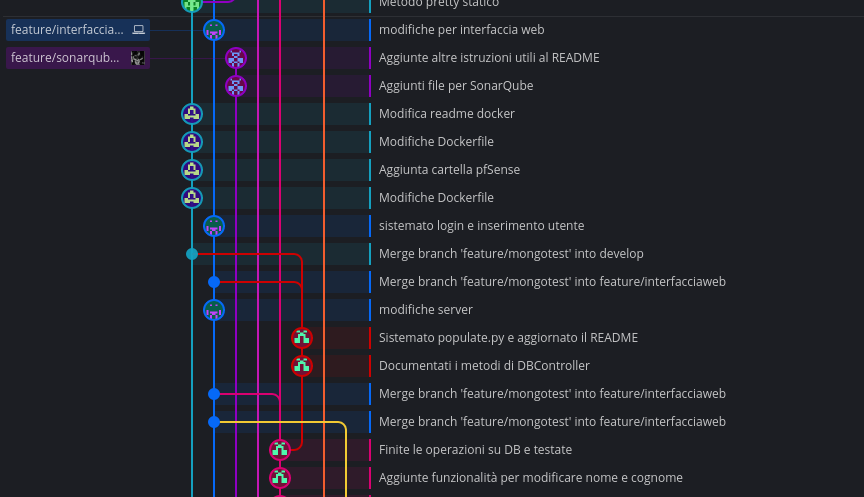
\includegraphics[width=\textwidth]{img/branches.png}\\
				\caption[Albero dei branch da Gitkraken]{Visione generale dell'albero dei branch in un momento casuale da Gitkraken}
				\label{fig:butterfly}
			\end{figure}

		\subsubsection{Controllo della configurazione} \label{ControlloConfigurazione}
		Per il controllo e l'approvazione dei cambiamenti alle repository adottiamo le seguenti regole.
		È cura del \Ver\ controllare che vengano rispettate.

			\paragraph{Aggiornamento della repository}
			Per aggiornare la repository remota con i cambiamenti effettuati nella workcopy locale, la prassi da seguire è la seguente:
			\begin{itemize}
				\item Controllare di trovarsi nel branch corretto con il comando:
					\begin{quote}
						\texttt{\$\ git branch}
					\end{quote}
					In caso negativo, dare il comando \texttt{git checkout nomebranch} per spostarsi nel branch corretto prima di procedere.
				\item Aggiornare la workcopy locale con eventuali cambiamenti presenti nella repository remota:
					\begin{quote}
						\texttt{\$\ git pull}
					\end{quote}
				\begin{itemize}
					\item In caso di conflitti, dare la sequenza di comandi che segue per risolverli senza dover effettuare un commit
						dedicato solo al merge:
						\begin{quote}
							\texttt{\$\ git stash}\par
							\texttt{\$\ git pull}\par
							\texttt{\$\ git stash pop}\par
						\end{quote}
						A questo punto, si potrebbero avere dei conflitti marcati opportunamente da Git, oppure avere la copia aggiornata
						con le proprie modifiche applicate.
				\end{itemize}
				\item Aggiungere i file allo ``stage'' relativi a una specifica modifica con il comando (è possibile usare * come wildcard
					per aggiungere più file contemporaneamente):
					\begin{quote}
						\texttt{\$\ git add [nome-file1] [nome-file2] \dots}
					\end{quote}
				\item Fare il commit e riassumere i cambiamenti apportati:
				\begin{quote}
					\texttt{\$\ git commit -m "Cambiamenti apportati"}
				\end{quote}
				\item Effettuare il push per pubblicare le modifiche locali nella repository remota:
				\begin{quote}
					\texttt{\$\ git push}
				\end{quote}
			\end{itemize}

	% 6.2.5.1 The following shall be determined and ensured: the functional completeness of the software items against their requirements and the physical completeness of the software items (whether their design and code reflect an up-to-date technical description).
	\subsubsection{Valutazione della configurazione}
	\label{ValutazioneConfigurazione}
	Per valutare la completezza delle funzionalità fornite da \progetto\ facciamo riferimento ai test di validazione presenti nel \PdQd.
	Per quel che riguarda la progettazione e il codice ci basiamo sul feedback ottenuto dal committente tramite la Product Baseline. Grazie ad esso infatti ci interroghiamo sulla conformità della nostra progettazione software.

	\subsubsection{Gestione del rilascio e consegna}	\label{GestioneRilascio}
	La consegna del prodotto finale avverrà al termine del progetto tramite un supporto fisico dato direttamente al committente.


	\subsection{Quality assurance}	\label{QualityAssurance}
	Il processo di \gloss{quality assurance} ci fornisce l'adeguata certezza che il nostro prodotto software e processi siano conformi ai loro specifici requisiti e che aderiscano ai piani stabiliti per essi.

		\subsubsection{Implementazione del processo} \label{ImplementazioneQA}
		Il nostro piano, che determina come i processi e i compiti di quality assurance devono essere sviluppati e implementati, è delineato nel \PdQd.
		Esso include:
		\begin{itemize}
			\item Standard di qualità, metodologie, procedure e strumenti per eseguire attività di quality assurance
			% \item 6.3.1.3 Procedures for contract review and coordination thereof
			\item Procedure per l'identificazione, raccolta, archiviazione e mantenimento dei risultati di qualità
			\item Risorse e programma per condurre le attività di quality assurance
		\end{itemize}

		\newpage

\section{Standard di qualità}	\label{standard di qualità}
Prendiamo come riferimento per gli obiettivi di qualità del prodotto determinati standard.


In questa appendice descriviamo gli standard adottati nelle loro parti più rilevanti ai fini del progetto. Nelle \NdPd\ viene indicato in che misura questi standard saranno applicati e nel \PdQd\ il piano che abbiamo scelto per rispettarli.

	\subsection{ISO/IEC 15504 (SPICE)}\label{iso15504}
	Lo standard ISO/IEC 15504 è stato creato per unire in un unico standard le caratteristiche principali di \gloss{CMMI} e \gloss{SPY}; entrambi standard riguardanti la qualità di processi software.
	ISO/IEC 15504 è chiamato anche SPICE come acronimo di \textit{Software Process Improvement and Capability Determination}, dando importanza al termine ``Capability'' inteso come la capacità di un processo di essere cognitivamente capace di raggiungere il suo scopo. 
	
	Un processo con un'alta Capability è osservato da tutti in modo disciplinato e sistematico.
	In caso di bassa Capability il processo viene effettuato in modo opportunistico e disorganizzato.\\
	
	SPICE mette a disposizione una metrica per valutare diversi attributi per ogni processo ed assegna un valore quantificabile ad ognuno di questi in modo tale da rendere esplicito come poter migliorare tale processo. Ogni valutazione in questo modo può essere ripetibile, oggettiva e comparabile.
	
	I processi vengono classificati in:

	

	\begin{itemize}
		\item Cliente/Fornitore
		\item Ingegneria
		\item Supporto
		\item Gestione
		\item Organizzazione
	\end{itemize}
	
	I livelli sono:
	
	\begin{itemize}
		\item \textbf{0 Incompleto}: il processo è caotico perché con risultati e performance incomplete.
	
		\item \textbf{1 Performato}: il processo inizia ad essere eseguito mettendo a disposizione degli input ed output.
		
		Attributi:
		
		\begin{itemize}
			\item \textbf{Esecuzione dei processi}: indica il numero di obiettivi raggiunti.
		\end{itemize}
	
		\item \textbf{2 Gestito}: le responsabilità e la gestione del processo sono definite.
		
		Attributi:
		
		\begin{itemize}
			\item \textbf{Gestione del processo}: indica quanto sono organizzati gli obiettivi fissati.
			\item \textbf{Gestione del prodotto}: indica quanto sono organizzati o gestiti i prodotti rilasciati.
		\end{itemize}
	
		\item \textbf{3 Stabilito}: il processo è pronto per diventare un processo standard ed essere rilasciato.
		
		Attributi:
		
		\begin{itemize}
			\item \textbf{Definizione del processo}: indica quanto il processo aderisce agli standard.
			\item \textbf{Distribuzione del processo}: indica in che misura il processo possa essere rilasciato potendo restituire sempre lo stesso risultato.
		\end{itemize}
	
		\item \textbf{4 Prevedibile}: il processo è in grado di essere sottoposto a metriche e valutazioni quantitative. Spesso i risultati sono predicibili.
		
		Attributi:
		
		\begin{itemize}
			\item \textbf{Misurazioni del processo}: indica quanto le metriche possono essere applicate al processo.
			\item \textbf{Controllo del processo}: indica quanto i risultati delle valutazioni siano predicibili.
		\end{itemize}
	
		\item \textbf{5 Ottimizzante}: il processo attua miglioramenti qualitativi e quantitativi.
		
		Attributi:
		
		\begin{itemize}
			\item \textbf{Innovazione del processo}: indica quanto i cambiamenti attuati nel processo risultino innovativi e positivi grazie ad una fase di analisi.
			\item \textbf{Ottimizzazione del processo}: indica quanto la curva di miglioramento del processo sia lineare.
		\end{itemize}
	\end{itemize}
	
	Ad ogni attributo viene data una valutazione assegnata in base alla percentuale di soddisfacimento dell'attributo:
	
	\begin{itemize}
		\item \textbf{N}: il processo non è implementato e non svolge niente di significativo (0\%-15\%).
		\item \textbf{P}: il processo è parzialmente implementato (15\%-50\%).
		\item \textbf{L}: il processo è largamente implementato (50\%-85\%).
		\item \textbf{F}: il processo è completamente implementato (85\%-100\%).
	\end{itemize}
	
\begin{table}[H]
	\centering
	\begin{oldtabular}{ccccc}
		\toprule
		\multirow{2}{*}{Attributi} & \multicolumn{4}{c}{Valutazioni}\\
		\cmidrule(lr){2-5} & N & P & L & F\\
		\midrule Esecuzione dei processi & \multicolumn{4}{c}{[0-1]}\\
		% Esecuzione dei processi & \multicolumn{4}{c}{[0-1]}\\
		\midrule Gestione del processo & \multicolumn{4}{c}{\multirow{2}{*}{[1-2]}}\\
		Gestione del prodotto\\
		\midrule Definizione del processo & \multicolumn{4}{c}{\multirow{2}{*}{[2-3]}}\\
		Distribuzione del processo\\
		\midrule Misurazione del processo & \multicolumn{4}{c}{\multirow{2}{*}{[3-4]}}\\
		Controllo del processo\\
		\midrule Innovazione del processo & \multicolumn{4}{c}{\multirow{2}{*}{[4-5]}}\\
		Ottimizzazione del processo\\
		\bottomrule
	\end{oldtabular}
	\label{tab:spice}
	\caption{Schema degli attributi di ISO/IEC 15504}
	\end{table}

%FIXME: dire a che minghie serve sta roba e quali punti in particolare
	\subsection{ISO/IEC 9126:2001}
	ISO/IEC 9126 è uno standard inerente alla qualità del software. Esso è strutturato in modo tale che si possa migliorare l'insieme dei processi.
	
	La sua struttura prevede tre tipi di qualità, ognuna delle quali possiede determinate caratteristiche:
	
	\begin{itemize}
		\item \textbf{Qualità interna}: misura la qualità di chi causa l'esecuzione del prodotto, in questo caso parliamo del codice sorgente a chi si possono assegnare diverse metriche attraverso l'analisi statica che ne stabiliscono poi la portabilità e la manutenibilità.
		
		Gli attributi ad essa assegnati sono:
		
		\begin{itemize}
			\item Manutenibilità
			\item Portabilità
		\end{itemize}
	
		\item \textbf{Qualità esterna}: misura attraverso l'analisi dinamica quanto l'esecuzione del prodotto rispetti gli obiettivi prefissati.
		
		Gli attributi ad essa assegnati sono:
		
			\begin{itemize}
			\item Funzionalità
			\item Efficienza
			\item Affidabilità
			\item Usabilità
		\end{itemize}
	
		\item \textbf{Qualità in uso}: definisce le metriche del prodotto rilasciato ed usato dal cliente che ne misurerà la qualità.
		
		Gli attributi ad essa assegnati sono:
		
		\begin{itemize}
			\item Efficacia
			\item Produttività
			\item Soddisfazione
			\item Safety
		\end{itemize}
	\end{itemize}

		\subsubsection{Descrizione degli attributi della qualità interna e della qualità esterna}
		\begin{itemize}
			\item \textbf{Manutenibilità}: il software nel corso delle sue revisioni deve essere facilmente modificabile.
			
			Nello specifico si prevede:
			
			\begin{itemize}
				\item \textbf{Analizzabilità}: prevedere una lettura del codice fruibile.
				\item \textbf{Modificabilità}: poter capire subito dove applicare la modifica.
				\item \textbf{Stabilità}: evitare effetti indesiderati dopo le modifiche.
				\item \textbf{Testabilità}: poter creare facilmente dei test su tutto il codice.
			\end{itemize}
		
			\item \textbf{Portabilità}: il software dovrebbe poter essere eseguito in più ambienti.
			
			Nello specifico si prevede:
			
			\begin{itemize}
				\item \textbf{Adattabilità}: potersi adattare automaticamente ai vari ambienti:
				\item \textbf{Installabilità}: la sua fase d'installazione dovrebbe essere semplice.
				\item \textbf{Conformità}: il software deve sapere coesistere con le altre applicazioni.
				\item \textbf{Sostituibilità}: essere capace di sostituire un software con gli stessi scopi.
			\end{itemize}
		
			\item \textbf{Funzionalità}: il software deve mettere a disposizione le funzionalità richieste in rapporto all'ambiente d'esecuzione.
			
			Nello specifico si prevede:
			
			\begin{itemize}
				\item \textbf{Appropriatezza}: le funzionalità del software sono appropriate ai requisiti richiesti.
				\item \textbf{Accuratezza}: in che misura le funzionalità aderiscono ai requisiti richiesti.
				\item \textbf{Interoperabilità}: la capacità di interagire coi sistemi specificati.
				\item \textbf{Security}: proteggere le informazioni da agenti esterni.
			\end{itemize}
		
			\item \textbf{Efficienza}: misura della capacità di raggiungere gli obiettivi stabiliti cercando di usare meno risorse possibili, in particolare:
			
			\begin{itemize}
				\item \textbf{Nel tempo}: poter dare risposte in un tempo di scadenza appropriato.
				\item \textbf{Nello spazio}: utilizzo del minor numero di risorse.
			\end{itemize}
		
			\item \textbf{Affidabilità}: il software deve mantenere le specifiche richieste senza inconvenienti.
			
			Nello specifico si prevede:
			
			\begin{itemize}
				\item \textbf{Maturità}: indica il livello minimo delle parti del prodotto che determina poi il livello di qualità dell'intero prodotto.
				\item \textbf{Robustezza}: la capacità di saper reagire agli errori.
				\item \textbf{Recuperabilità}: per poter tornare alla versione precedente del software in modo semplice.
			\end{itemize}
		
			\item \textbf{Usabilità}: il software deve poter essere compreso fin da subito, dunque semplice ed immediato nell'utilizzo e comprensione.
			
			Nello specifico si prevede:
			
			\begin{itemize}
				\item \textbf{Comprensibilità}: il significato delle funzionalità deve essere compreso il prima possibile dall'utente.
				\item \textbf{Apprendibilità}: capacità di saper usare le funzionalità disponibili.
				\item \textbf{Operabilità}: capacità dell'utente di usare e controllare il software.
				\item \textbf{Attrattiva}: il risultato deve risultare attraente all'utente.
			\end{itemize}
		\end{itemize}
	
		\subsubsection{Descrizione degli attributi della qualità in uso}
		\begin{itemize}
			\item \textbf{Efficacia}: misura della capacità di riuscire a raggiungere i compiti fissati. Essa si calcola
			in base al grado di raggiungimento degli obiettivi.
			\item \textbf{Produttività}: intesa come $ \frac{\text{unità di prodotto realizzato}}{\text{unità di risorse utilizzate}} $.
			\item \textbf{Soddisfazione}: il software deve soddisfare l'utente.
			\item \textbf{Safety}: il software deve possedere adeguati livelli di sicurezza per il tipo di utente che ne usufruisce.
		\end{itemize}
	
	\begin{figure}[H]
		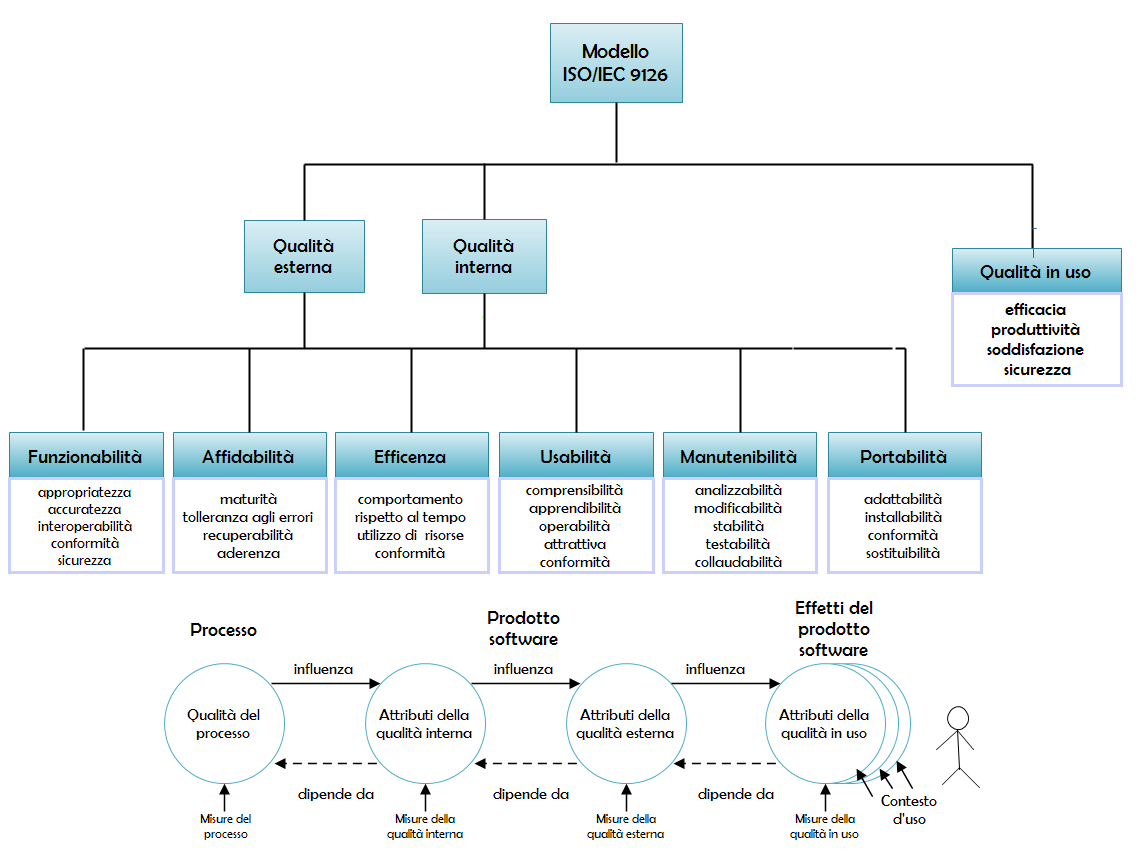
\includegraphics[width=\textwidth]{img/ISO9126_full.png}
		\label{fig:iso9126}
		\caption[Schema ISO 9126 con il suo ciclo di vita]{Schema ISO 9126 con il suo ciclo di vita\protect\footnotemark}
	\end{figure}

	\footnotetext{Vedere in \S\ref{riferimenti informativi}}
	
	\subsection{Ciclo di Deming}	\label{cicloDeming}
	Il Ciclo di Deming è un metodo iterativo creato per migliorare la qualità dei processi e dei prodotti software. È un metodo che opera nell'ottica di un miglioramento continuo in termini di risultati e risorse utilizzate e al termine di ogni ciclo, l'eventuale miglioramento effettuato diventa la nuova base da cui inizia l'iterazione successiva.
	
	Si distingue in quattro fasi, chiamate anche PDCA, che sono:
	
	\begin{itemize}
		\item \textbf{Plan}: pianificare i processi per ottenere i risultati attesi ed osservare dove questi possono essere migliorati.
		\item \textbf{Do}: eseguire il programma e i miglioramenti inseriti nella fase precedente.
		\item \textbf{Check}: effettuare test e controlli dell'output della fase precedente confrontandoli con gli obiettivi della fase di Plan. Dare una valutazione dei risultati per verificare se i cambiamenti attuati portano effettivamente dei miglioramenti.
		\item \textbf{Act}: le modifiche, se risultano essere delle migliorie vengono applicate al processo o al prodotto.
	\end{itemize}

	\begin{figure}[H]
		\centering
		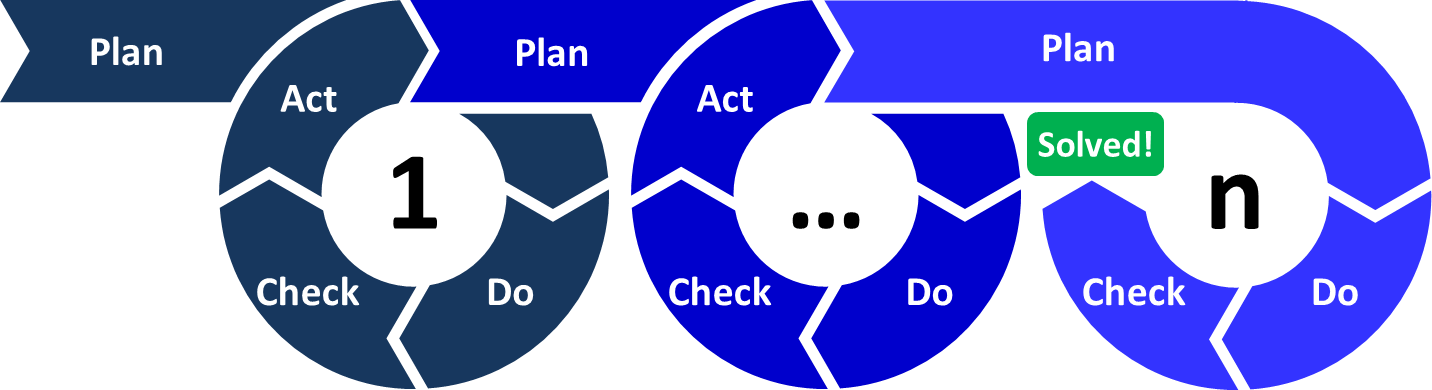
\includegraphics[width=0.65\textwidth]{img/PDCA}
		\label{fig:PDCA}
		\caption[Ciclo di Deming]{Ciclo di Deming\protect\footnotemark}
	\end{figure}

	\footnotetext{Vedere Riferimenti Informativi in \S\ref{riferimenti informativi}}

	\subsection{ISO/IEC 90003:2004}
	Lo standard ISO/IEC 90003 consiste nello standard ISO 9001:2008 applicato al software. Quest'ultimo tratta di uno standard sulla qualità dei sistemi aziendali che segue il sistema il Ciclo di Deming descritto in \S\ref{cicloDeming}.
	
	L'ISO/IEC 90003:2004 si suddivide in otto capitoli che sono:
	
	\begin{enumerate}
		\item Scopo
		\item Riferimenti normativi
		\item Termini e definizioni
		\item Sistema di gestione della qualità
		\item Gestione delle responsabilità
		\item Gestione delle risorse
		\item Realizzazione del prodotto
		\item Misurazione, analisi e miglioramento
	\end{enumerate}

	Date le nostre capacità e la nostra esperienza, prendiamo in considerazione solo alcuni punti del quarto capitolo. In particolar modo quelli riguardanti la documentazione, non potendo ancora stabilire metriche sul software.
	
	\subsubsection{Capitolo 4. dell'ISO 90003: requisiti di sistema e linee guida}
	
	\begin{enumerate}
		\item \textbf{Requisiti e linee guida sull'organizzazione}:
		\begin{enumerate}
			\item \textbf{Stabilire la gestione del sistema di qualità (QMS)}
			\begin{itemize}
				\item \textbf{Identificare i requisiti di cui il QMS ha bisogno}: attraverso il \PdQ~osservando i processi interni ed esterni.
				\item \textbf{Assicurarsi che ogni processo sia efficacie}: attraverso una verifica continua sui processi e prodotti.
			\end{itemize}
			\item \textbf{Documentare il proprio QMS}: riportare le relazioni tra i vari processi e come essi vengano gestiti e verificati.
			\item \textbf{Cercare di migliorare il proprio QMS}: applicando il ciclo di Deming.
			\item Mantenere la qualità del QMS
		\end{enumerate} 
		
		\item \textbf{Requisiti e linee guida sulla documentazione}:
		\begin{enumerate}
			\item \textbf{Documentare la qualità}:
			\begin{itemize}
				\item \textbf{Pianificare la documentazione del QMS}: assicurandosi che quello che verrà scritto rispecchi gli obiettivi e la gestione dei processi.
				\item \textbf{Stabilire la documentazione del QMS}: stabilendo la qualità delle diverse parti del QMS.
				\item Mantenere la documentazione nel tempo
			\end{itemize}
			
			\item \textbf{Controllare la qualità dei documenti}:
			\begin{itemize}
				\item \textbf{Stabilire una procedura per controllare i documenti}: documentare la stessa procedura di controllo che dovrebbe contenere la fase di approvazione del documento, un suo versionamento e continuo aggiornamento.
				\item Mantenere ed aggiornare la procedura di controllo del documento
			\end{itemize}
		\end{enumerate}
	\end{enumerate}


		\subsubsection{Attività}	\label{AttivitaPDQ}
		Nello specifico, le attività trattate dal \PdQd\ sono:
		\begin{itemize}
			\item Qualità di processo
			\item Qualità di prodotto
			\item Resoconto delle attività di verifica
			\item Mitigazione delle variazioni orarie
			\item Valutazione per il miglioramento
		\end{itemize}



	\subsection{Verifica}\label{Verifica}

		\subsubsection{Scopo}
		Questa sezione vuole descrivere come eseguiamo la fase di verifica, lo scopo è quello di evidenziare
		ed eliminare la presenza di errori nell’esecuzione di un qualunque processo durante tutto lo sviluppo del prodotto.

		%\subsubsection{Aspettative} %da mettere nel PdQ

		\subsubsection{Descrizione}
		Ogni processo e prodotto deve essere valutato in modo quantificabile attraverso metriche apposite, quando possibile, e stabilendo il risultato che si vuole
		raggiungere.

		Come indicato dal \gloss{Ciclo di Deming}, nel momento in cui tale risultato sarà raggiunto, se esso non è il migliore,
		servirà come ``base'' per alzare il livello di qualità di quel processo o prodotto.

		I risultati ottenuti nella fase di verifica sono riportati nel \PdQd: in questo modo, confrontandoli con gli esiti attesi,
		è possibile valutare un miglioramento per i vari processi e prodotti.

		\subsubsection{Walkthrough e Inspection}
		Due modi di effettuare la verifica sono attraverso Walkthrough e Inspection.
		Li adotteremo entrambi, ma non contemporaneamente, per i vantaggi che comporta ogni metodo.

			\paragraph{Walkthrough}
			Metodo di verifica che effettua un controllo ad ampio spettro senza l’assunzione di presupposti. Dato che per mettere in atto tale metodo ci
			si deve dividere in gruppi dove ognuno ha un ruolo ben distinto, Walkthrough è ideale per le verifiche effettuate all'inizio dei vari periodi,
			dove i membri del team di sviluppo non possiedono le conoscenze adeguate per una verifica efficiente.

			Walkthrough possiede delle fasi ben specifiche:

			\begin{enumerate}
				\item \textbf{Pianificazione}: viene pianificato in gruppo come effettuare la verifica dei prodotti.
				\item \textbf{Lettura}: viene effettuata la lettura del prodotto.
				\item \textbf{Discussione}: vengono discusse le possibili correzioni.
				\item \textbf{Correzione di difetti}: si attuano i risultati ottenuti dalla fase di discussione.
			\end{enumerate}

			\paragraph{Inspection}
			Metodo di verifica dove si esegue una lettura mirata dei prodotti, frutto di un'analisi dei risultati dei precedenti test.
			Questo metodo dunque, a differenza di Walkthrough, prevede l'esecuzione con dei presupposti.

			Le fasi di Inspection sono:

			\begin{enumerate}
				\item \textbf{Pianificazione}: viene sempre deciso in gruppo come effettuare la pianificazione.
				\item \textbf{Definizione di una lista di controllo}: dato che le parti da verificare sono specificate, queste possono essere
				riportate in una lista in modo da velocizzare il processo di verifica.
				\item \textbf{Correzione dei difetti}: attuazione dei punti della lista di controllo.
			\end{enumerate}

			Per la natura di Inspection, questa non può essere applicata fin dall'inizio, dunque nel momento in cui si presentano nuove tipologie di
			prodotti e processi da verificare viene effettuato Walkthrough; nel momento in cui il metodo di verifica è ben consolidato da tutti noi,
			si passa ad effettuare verifica secondo Inspection.

		\subsubsection{Verifica del design e conformità del codice}	\label{VerificaDesign}
		Il \Ver\ ha il compito di verificare la progettazione.
		In particolare si occupa di:
		\begin{itemize}
			\item Controllare che i design pattern che abbiamo scelto vengano effettivamente rappresentati nella maniera corretta tramite i diagrammi e che rispettino gli obiettivi preposti
			\item Verificare che il codice sviluppato sia coerente con quanto dichiarato nella progettazione
		\end{itemize}


		\subsubsection{Metodologie di sviluppo del software}

		\paragraph{The Twelve-Factor App}
		\gloss{The Twelve-Factor App} è una serie di dodici regole destinate a chi vuole sviluppare \gloss{software-as-a-service} (SaaS). Sono utili per verificare in corso d'opera la qualità del progetto, valutando quali punti riesce a rispettare l'applicazione.

		I suoi principi sono:

		\begin{enumerate}
			\item \textbf{\gloss{Codebase}}: deve essere presente una sola codebase versionata da un \gloss{Version Control System} (VCS) come \gloss{GitLAb} da cui
			possono derivare diversi \gloss{deploy}.
			\item \textbf{Dipendenze}: le librerie usate dal codice devono essere presenti nella directory della singola applicazione e non attive a livello di \gloss{sistema}. In questo modo l'applicazione è il meno dipendente possibile dal sistema di esecuzione.
			\item \textbf{Configurazione}: i parametri di configurazione dell'applicazione devono essere completamente separati dalla sua implementazione.
			\item \textbf{Backing Service}: l'applicazione non deve far distinzione tra funzionalità uguali usate in locale o remoto.
			\item \textbf{Build, release, esecuzione}: bisogna separare in modo netto la fase di build, quella di deploy e quella esecuzione, usando \gloss{tool} differenti e diverse repository per salvare i risultati delle varie fasi.
			\item \textbf{Processi}: l'esecuzione dell'applicazione deve essere vista come l'insieme di uno o più processi che restituiscono un risultato. Questi sono di tipo \gloss{stateless}.
			\item \textbf{\gloss{Binding} delle Porte}: l'applicazione è completamente contenuta in se stessa e non fa affidamento ad un altro servizio nell'ambiente di esecuzione. Effettua invece il binding delle porte diventando un servizio per le richieste esterne.
			\item \textbf{Concorrenza}: sviluppare i processi in modo tale che possano lavorare su un sistema decentralizzato.
			\item \textbf{Rilasciabilità}: i processi dell'applicazione devono poter essere avviati e fermati quando se ne ha bisogno senza passaggi bruschi.
			\item \textbf{Parità tra sviluppo e produzione}: deve esserci meno differenza possibile tra lo stato di sviluppo e quello di produzione. Questo si ottiene facendo un rilascio continuo del prodotto.
			\item \textbf{Log}: l'applicazione dovrebbe poter offrire un sistema di login.
			\item \textbf{Processi di Amministrazione}: porre attenzione a quei processi che devono essere eseguiti una tantum dagli sviluppatori ad esempio. Questi processi devono poter essere accessibili solo ad alcuni e indicati in una specifica release.
		\end{enumerate}

		In accordo col cliente \II, non tutti i punti di Twelve-Factor App possono essere rispettati. In particolare non è richiesto il soddisfacimento del punto 12, mentre il punto 11 è lasciato al fornitore come opzionale.

		\paragraph{Test Driven Development}\label{tdd}
		Come metodologia di sviluppo del software adottiamo il Test Driven Development (TDD) per ogni componente.
		Questa metodologia prevede tre fasi nello sviluppo che, ripetute ciclicamente, costituiscono il Ciclo TDD:
		\begin{itemize}
			\item \textbf{Fase rossa}: il \Progr\ scrive il test relativo alla funzionalità che vuole implementare, prima di scrivere
				il nome del metodo o la sua implementazione. Questo porterà ad un fallimento assicurato poiché il metodo non esiste o non fa nulla.
			\item \textbf{Fase verde}: il \Progr\ scrive il codice della funzionalità minimo indispensabile a far superare il test.
			\item \textbf{Fase grigia (Refactoring)}: il \Progr\ riscrive il codice per far sì che il codice rispetti
				gli obiettivi di qualità definiti nel \PdQd\ e al contempo superi il test.
		\end{itemize}

		\begin{figure}[H]
			\centering
			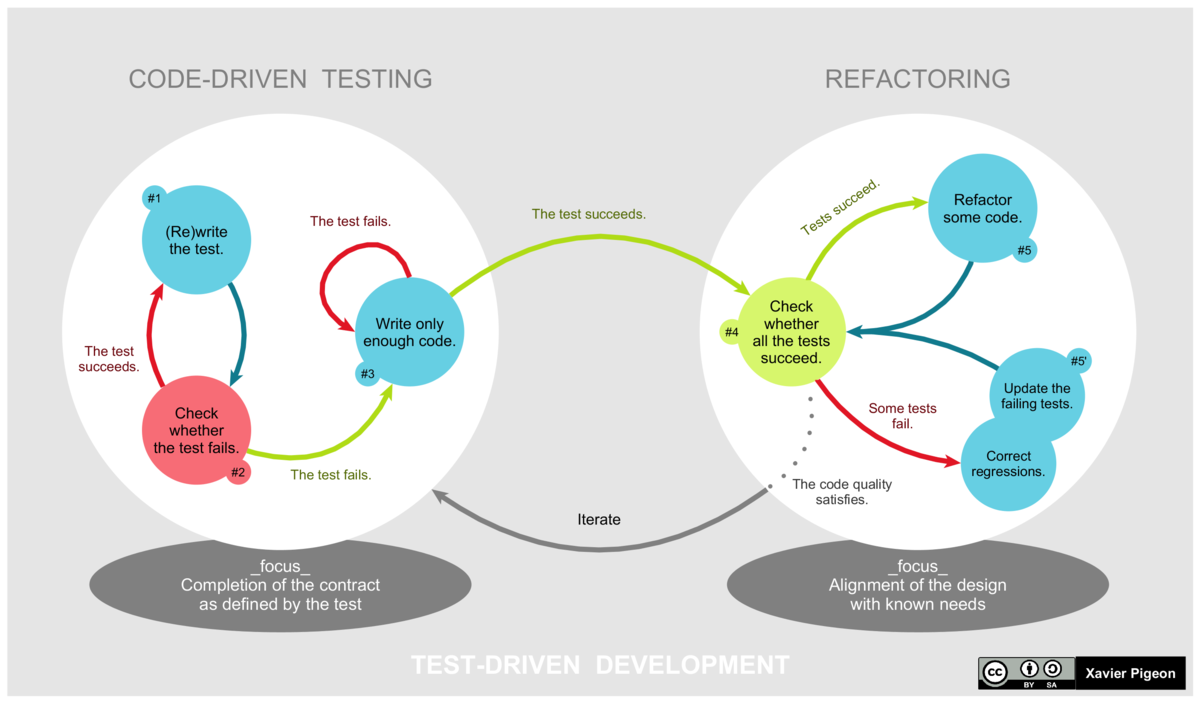
\includegraphics[width=\textwidth]{img/tdd.png}\\
			\caption[Test Driven Development]{Test Driven Development\protect\footnotemark}
			\label{TDDfigure}
		\end{figure}

		\footnotetext{Riferirsi alla voce
		%``Fonte Figura 3''
		7
		 in \S\ref{rifinfo}}

		\subsubsection{Analisi statica}\label{AnalisiStatica}
		L'analisi statica attua una verifica non dinamica, ovvero senza eseguire codice.
		Può essere effettuata sui documenti o sul codice in maniera statica.


			\paragraph{Analisi dei documenti}\label{ProcessiSupportoMetriche}
			L'analisi statica per i documenti si limita a valutare come e con che contenuti questi vengono scritti.
			Per l'analisi dei documenti vengono utilizzate due metriche:

			\begin{itemize}
				\item MPD001
				\item MPD002
			\end{itemize}

			La denominazione delle metriche è descritta in \S\ref{Classificazione metriche}.

			\subparagraph{MPD001 Indice di Gulpease}\label{AnalisiStatica:Gulpease}
			Per il calcolo dell'indice di Gulpease, abbiamo creato uno script ad hoc che, preso in input un file PDF, produce in output l'indice di Gulpease.
			L'indice si calcola:

			\[89+\dfrac{300\times n_{\text{frasi}}-10\times n_{\text{lettere}}}{n_{\text{parole}}}\]

			\textbf{Metrica}: il risultato della formula è interpretato nel seguente modo

			\begin{itemize}
				\item \textbf{<80}: documento  difficile da leggere per chi ha la licenza elementare.
				\item \textbf{<60}: documento  difficile da leggere per chi ha la licenza media.
				\item \textbf{<40}: documento difficile da leggere per chi ha un diploma superiore.
			\end{itemize}

			Nel momento in cui avviene un commit all'interno di repository, in automatico si avvia uno script che analizza tutti i documenti in PDF per valutarne
			l'indice di Gulpease. I risultati vengono poi riportati in un apposito file di testo per verificarne la qualità ed un possibile miglioramento.

			\subparagraph{MPD002 Correttezza ortografica}\label{AnalisiStatica:CorrettezzaOrtografica}
			Gli errori ortografici possono essere segnalati dallo strumento di Controllo Ortografico presente in \textit{TexStudio} e da GNU Aspell.

			\textbf{Metrica}: il numero di errori ortografici presenti nel documento.


			\paragraph{Analisi dei processi}\label{analisipr}
			Per analizzare i processi usiamo gli standard sopra elencati. Ad ogni fase del processo, verranno valutati gli attributi richiesti secondo
			l'ISO 15504, in che misura questi sono stati rispettati e in che fase del Ciclo di Deming il processo si trova.
			Per l'analisi dei processi vengono utilizzate:

			\begin{itemize}
                \item MPR003 Aderenza agli standard
				\item MPR004 Frequenza commit nella repository
				\item MPR009 Frequenza controllo prodotti
				\item MPR010 Moduli codificati prima della progettazione
                \item MPR011 Numero di design pattern applicati
                \item MPR012 Moduli non testati
			\end{itemize}

			La denominazione delle metriche è descritta in \S\ref{Classificazione metriche}.

            \subparagraph{MPR003 Aderenza agli standard}
            Per misurare e verificare i processi sono stati scelti alcuni specifici standard di qualità descritti nel \PdQd\ che possono offrire una valutazione quantitativa.
            Gli standard scelti sono:

            \begin{itemize}
                \item \textbf{ISO/IEC 15504}: ogni processo attivato verrà classificato e valutato secondo gli attributi assegnati ai vari livelli di qualità. Per ogni attributo verrà infine indicata una percentuale di quanto il processo rispetti l'attributo, potendo infine capire nel complesso quanto quel processo riesca a superare un dato livello di maturità.
                \item \textbf{Ciclo di Deming}: nella fase migliorativa del processo sarà data particolare attenzione nel non iniziare una fase del Ciclo di Deming senza aver finito completamente le fasi precedenti.
            \end{itemize}

	        \textbf{Metrica}: il livello di maturità è descritto in appendice A.1 del \PdQd.

			\subparagraph{MPR004 Frequenza commit nella repository}
			Per mantenere aggiornate le versioni dei prodotti è necessario che ognuno di noi effettui un commit ad ogni sua modifica significativa.
			Così facendo, in caso di errori, è possibile tornare ad una versione stabile del progetto.
			Misurare quanti commit sono stati effettuati inoltre serve per monitorare l'attività del team di sviluppo.
			\[\dfrac{\sum_{i=1}^{n} x_i}{n} \qquad x_i=\text{numero di commit alla i-esima settimana del macro periodo.}\]
			\textbf{Metrica}: numero minimo di commit da effettuare in media ogni settimana lavorativa durante un macro-periodo.


			\subparagraph{MPR009 Frequenza controllo prodotti}
			I documenti e i prodotti software hanno bisogno di una verifica frequente, commisurata in base al numero di modifiche che vengono apportate.

			Chi esegue la modifica deve controllare ciò che ha fatto prima di poterla ufficializzare, mentre la verifica fatta dal \Ver\ deve essere
			fatta solo nel momento in cui è stato raggiunto un numero significativo di modifiche, per evitare di spendere troppe risorse in questa fase.

			\[\dfrac{\sum_{i=1}^{n} x_i}{n} \qquad x_i=\text{numero di modifiche effettuate prima della i-esima verifica.}\]

			\textbf{Metrica}: media del numero massimo di modifiche apportate ai prodotti prima che ricevano una verifica dal parte del \Ver.

            \subparagraph{MPR010 Moduli codificati prima della progettazione}
            La progettazione di un \gloss{modulo} è fondamentale per rendere il prodotto estensibile, mantenibile e comprensibile. Per questo è buona prassi avviare il processo di progettazione prima di quello di codifica.

            La progettazione di ogni modulo all'interno dell'intero prodotto software deve essere fatta prima della sua codifica, la quale deve rispecchiare la progettazione.

            \textbf{Metrica}: percentuale di moduli non progettati prima della loro codifica. Per fare ciò, nelle varie fasi di verifica, si contano i moduli codificati prima di essere progettati. Verso il termine del periodo di revisione si calcola la loro percentuale in base al numero totale di moduli prodotti.

            \subparagraph{MPR011 Numero di design pattern applicati}
            Dato che i design patter possono essere considerati una ``buona pratica'' per produrre del codice in determinati contesti, la loro presenza può aiutare ad innalzare la qualità del prodotto. Il loro uso massiccio però può portare ad un'eccessiva complessità e talvolta anche ad un mal funzionamento del prodotto se applicati erroneamente; per questo i design pattern devono essere applicati in maniera ponderata.

            \textbf{Metrica}: numero di volte che si applica uno o più tipi di design pattern.

            \subparagraph{MPR012 Moduli non testati}
            Dobbiamo sempre testare i \gloss{moduli} per assicurarci la loro correttezza. Per fare ciò, devono essere testate le \gloss{unità} che li compongono attraverso i test di unità (definiti in \S\ref{testunita}).
            Ogni modulo deve dunque essere testato.

            \textbf{Metrica}: numero di moduli codificati e privi di test di unità.


			\paragraph{Analisi del software} \label{analisisw}
			L'analisi statica del codice, insieme alle norme di codifica stabilite in \S\ref{PP:Sviluppo:Codifica}, serve per permetterci di scrivere programmi verificabili.
			In particolare ci aiuta per assicurare un comportamento predicibile, per darci dei criteri di programmazione ben fondati da usare e per ragioni pragmatiche.
			Un potente mezzo che ci permette di eseguire analisi statica sul codice è \gloss{SonarQube}.
			Da esso, traiamo le seguenti metriche:
			\begin{itemize}
				\item MPS001 Presenza di bug
				\item MPS002 Presenza di vulnerabilità
				\item MPS003 Presenza di code smell
				\item MPS004 Duplicazione del codice
				\item MPS017 Code coverage
			\end{itemize}

			La denominazione delle metriche è descritta in \S\ref{Classificazione metriche}.

			\subparagraph{Controllo del Python coding style}\label{pycodestyle}
			Per l'analisi statica dello stile di codifica dei sorgenti Python, utilizziamo due strumenti che segnalano se lo stile di codifica non rispetta
			le norme definite nel PEP 8:
			\begin{itemize}
				\item \texttt{pycodestyle}: un tool che segnala, tramite comando da terminale, se e quali righe di codice di un file non rispettano lo standard PEP 8.
				\item \texttt{pylama}: un linter che segnala dinamicamente se ciò che viene digitato contiene degli errori o non rispetta
					lo standard PEP 8.
			\end{itemize}

			\subparagraph{SonarQube} \label{sonarqube}
			È una piattaforma open-source per realizzare controlli sulla qualità del codice tramite analisi statica.
			Lo utiliazziamo perché è possibile creare dei progetti che scansionano il nostro progetto locale e ci mostrano in una dashboard le attività più significative che lo strumento rileva.
			Si possono rilevare bug, \gloss{code smell}, duplicazione e vulnerabilità del codice.
			Viene inoltre assegnato una valore ``passato'' o ``non passato'' denominato Quality gate, che ci consente di valutare immediatamente la qualità generale del nostro codice.
			In particolare, SonarQube rispetto ad altri strumenti simili, ci è molto utile perchè supporta parecchi linguaggi di programmazione, tra cui quello che noi più utilizziamo: Python.

			\begin{figure}[H]
				\centering
				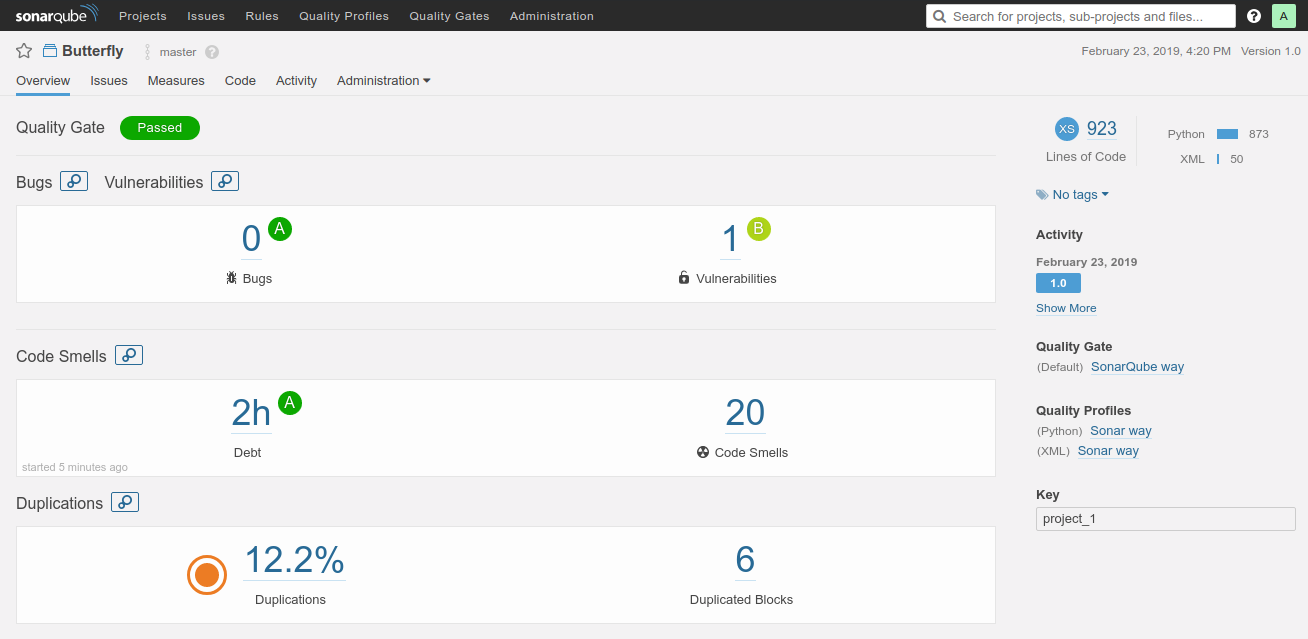
\includegraphics[width=\textwidth]{img/sonar.png}\\
				\caption[Screen SonarQube]{Esempio di immagine catturata del progetto Butterfly in SonarQube.}
				\label{fig:butterflySonar}
			\end{figure}

			\subparagraph{MPS001 Presenza di bug} \label{presenzabug}
			I bug sono difetti nel codice che vogliamo assolutamente tenere sotto controllo e rimuovere se rilevati.
			A questo scopo, SonarQube ci dà la possibilità di conteggiare il numero di bug presenti nel codice. \\
			\textbf{Metrica}: numero di bug presenti nel codice al momento della scansione.

			\subparagraph{MPS002 Presenza di vulnerabilità} \label{presenzavulnerabilita}
			Le vulnerabilità hanno un peso di gravità minore per noi, ma è comunque buona prassi cercare di minimizzarle il più possibile in modo da non incorrere in problemi di sicurezza.
			SonarQube ci dà la possibilità di visualizzare le vulnerabilità presenti nel codice. \\
			\textbf{Metrica}: numero di vulnerabilità presenti nel codice al momento della scansione.

			\subparagraph{MPS003 Presenza di code smell} \label{presenzacodesmell}
			I code smell non sono errori, ma indicano delle debolezze nel codice.
			La maggior parte di code smell segnalati da SonarQube, riguardano spesso linee di commenti che decrementano la leggibilità del codice.  \\
			\textbf{Metrica}: numero di code smell presenti nel codice al momento della scansione.

			\subparagraph{MPS004 Duplicazione del codice} \label{duplicazionecodice}
			Linee di codice duplicate segnalano inefficienza all'interno del nostro codice.
			Del buon codice infatti non è ridondante.
			Se lo è, vuol dire che può essere migliorato organizzandolo in modo differente.
			Per questo SonarQube ci dà la possibilità di visualizzare esattamente il numero percentuale di codice duplicato all'interno di un file, sul suo totale di righe. \\
			\textbf{Metrica}: percentuale di linee di codice duplicate presenti nel codice al momento della scansione.

            \subparagraph{MPS017 Code coverage} \label{codecoverage}
            Per sapere se un modulo è stato correttamente testato, si verifica in percentuale quante righe di codice vengono eseguite per superare una suite di test. Più è alta questa percentuale, più è bassa la probabilità che il codice contenga dei bug.

            \textbf{Metrica}: percentuale di \gloss{code coverage}.

		\subsubsection{Analisi dinamica}\label{AnalisiDinamica}
		L'analisi dinamica valuta il comportamento dei prodotti in esecuzione, verificando se restituiscono i risultati attesi e se operano nel modo stabilito.
		Vengono presi in esame i prodotti software e i processi.

		È oppurtono ricordare che i test devono essere:
		\begin{itemize}
			\item Ripetibili
			\item Automatizzati tramite strumenti
			\item Oggettivi e non personalizzati
		\end{itemize}

		Quindi, perché l'analisi dinamica avvenga in modo corretto, è necessario tenere conto di alcuni importanti elementi quali:
		\begin{itemize}
			\item \textbf{Ambiente di sviluppo}: il sistema hardware e software adottato durante il test.
			\item \textbf{Stato iniziale}: primo stato del prodotto, antecedente all'inizio del test.
			\item \textbf{Input}: dati inseriti.
			\item \textbf{Output}: dati attesi.
			\item \textbf{Notifica risultato}: notifiche riguardanti il risultato ottenuto dal test (opzionale).
		\end{itemize}

		Per effettuare analisi dinamica è necessario sviluppare dei dei test che verifichino l'integrità dei prodotti. Questi sono classificati attraverso un identificativo univoco descritto nel prossimo paragrafo e suddivisi per tipo in base alla tipologia dell'oggetto di test.

			\paragraph{Classificazione dei test}\label{ClassificazioneTest}
			Ogni test viene classificato identificato univocamente da tale codice:

			\begin{center}
				\texttt{T[Tipo][ID]}
			\end{center}

			\begin{itemize}
				\item \textbf{T}: si riferisce a ``Test''.
				\item \textbf{Tipo}: la tipologia a cui il test appartiene che, seguendo il modello a V%\footnote{\url{https://en.wikipedia.org/wiki/V-Model_(software_development)}}
				, può essere:
				\begin{itemize}
					\item \textbf{V}: validazione.
					\item \textbf{S}: sistema
					\item \textbf{I}: integrazione.
					\item \textbf{U}: unità.
				\end{itemize}
				%per la corrispondenza con i requisiti, non vanno bene le "tre cifre"
				\item \textbf{ID}: numero incrementale che rispetta una struttura gerarchica.
			\end{itemize}

			% COLORI
			\newcommand{\TNI}{{\color{gray}\textbf{NI}}}
			\newcommand{\TI}{{\color{blue}\textbf{I}}}
			\newcommand{\TNS}{{\color{red}\textbf{NS}}}
			\newcommand{\TS}{{\color{green}\textbf{S}}}

			Le tabelle che raccolgono i test di una determinata tipologia presentano i campi:
			\begin{itemize}
				\item \textbf{Codice}: comprendente il codice identificativo del test.
				\item \textbf{Test}: descrive cosa il test deve verificare.
				\item \textbf{Stato}: indica lo stato del test e può essere:
				\begin{itemize}
					\item \TNI: non implementato.
					\item \TI: implementato ma non ancora avviato.
					\item \TNS: avviato e fallito.
					\item \TS: avviato e superato.
				\end{itemize}
			\end{itemize}

			Ad esempio:

			\newenvironment{VTtable}[1][1]{%
				\renewcommand*{\arraystretch}{#1}%
				\renewcommand\theadfont{\bfseries}%
				\oldtabularx%
			}{\endoldtabularx}
			\newcounter{tv}
			\newcommand{\addtotv}{\stepcounter{tv}TV\thetv}
			\begin{table}[H]
				\begin{VTtable}[1.7]{\textwidth}{cXc}
					\rowcolor{\tablegray}
					\textbf{Codice} & \centering\textbf{Test} & \textbf{Stato} \\\toprule
					\addtotv & Verifica la segnalazione dell'apertura di una issue in Redmine \dots
					& \TNI \\
					\bottomrule
				\end{VTtable}
			\end{table}

			\paragraph{Test d'integrazione} \label{testintegrazione}
			I test d'integrazione verificano il residuo mettendo insieme due unità. Queste unità in particolare sono considerati indipendenti, ma realizzate al fine di essere composte per collaborare.
			Il test di integrazione ha tanti test quanti ne servono per accertarsi che tutti i dati scambiati attraverso ciascuna interfaccia siano conformi alla loro specifica e accertarsi che tutti i flussi di controllo previsti siano stati effettivamente provati.
			La strategia che i test d'integrazione adottano è una strategia di tipo incrementale: si basa nella prosecuzione per passi, aggiungendo parti fino al completamento.
			Più test eseguiamo, più è piccola la parte che stiamo testando. \\
			In una buona architettura, l'integrazione può anche essere parallelizzata.
			In particolare, la logica dell'integrazione funzionale segue i passi:
			\begin{itemize}
				\item Selezione delle funzionalità da integrare
				\item Identificazione delle varie componenti che svolgono quelle funzionalità
				\item Ordinamento delle componenti per numero di dipendenze crescenti
				\item Esecuzione dell'integrazione in quel determinato ordine
			\end{itemize}
			Inoltre rileva problemi quali:
			\begin{itemize}
				\item Errori residui nella realizzazione dei componenti
				\item Modifiche delle interfacce o cambiamenti nei requisiti
				\item Riuso di componenti dal comportamento oscuro o inadatto
				\item Integrazione con altre applicazioni non ben conosciute
			\end{itemize}

            \subparagraph{MPS019 Test di integrazione}\label{testintegrazione:met}
            La qualità di un prodotto si verifica attraverso la percentuale di test di integrazione superati.

            \textbf{Metrica}: percentuale di test di integrazione superati.

			\paragraph{Test di unità} \label{testunita}
			I test di unità sono l'attività di test di singole unità software.
			Per unità si intende il minimo componente di un programma dotato di funzionamento autonomo, ma non è semplice individuare l'unità.
			Va scelta durante l'attività di progettazione e deve essere sufficientemente piccola da facilitarne la verifica e la \gloss{liability}.

            \subparagraph{MPS020 Test di unità}\label{testunita:met}
            La qualità di un prodotto si verifica attraverso la percentuale di test di unità superati.

            \textbf{Metrica}: percentuale di test di unità superati.

			\paragraph{Test di regressione} \label{testregressione}
			I test di regressione sono una ripetizione selettiva dei test di unità, integrazione e sistema.
			La utilizziamo per assicurarci che una modifica fatta su un'unità per correggere un problema, non faccia danno ad altre causando regressione.
			Ciò avviene quando il sistema è altamente accoppiato.
			La regressione si riduce invece riducendo l'accoppiamento, per esempio tramite \gloss{incapsulamento}.

			\paragraph{Tracciamento dei test} \label{TracciamentoTest}
			Tutti i test da noi delineati presentano un tracciamento in forma tabellare con i requisiti o componenti applicativi a loro associati.
			Questo ci assicura una verifica più accurata e completa.


		\subsubsection{Anomalie riscontrate}\label{Anomalie}
		Durante i processi di verifica è possibile riscontrare a volte alcune anomalie.
		Tali anomalie posso essere dovute:
		\begin{itemize}
			\item A qualche valore preso come riferimento diverso da quello prestabilito per la metrica
			\item Al fallimento di un test
		\end{itemize}
		Ciò ci è utile perché un anomalia ci indica la presenza di errori nel prodotto o nel nostro way of working. Può quindi essere per noi un buon punto di inizio per la rivisitazione dei prodotti.
        
        %TODO da inserire nella sezione di validazione quando verrà divisa verifica e validazione
        \subsubsection{MPR013 Percentuale soddisfacimento metriche}\label{percentualeSoddisfacimentoMetriche}
        Al momento della consegna del prodotto al cliente è bene fare un'analisi retrospettiva del lavoro svolto, in modo da capire se il gruppo ha lavorato bene o meno, in modo da migliorarsi per i progetti futuri. \par
        Per calcolare tale metrica è necessario usare tutte le altre metriche:
        \[{\sum_{i=1} \frac{x_i}{y_i}}100\] $x_i=$ numero di volte che il valore della i-esima metrica è maggiore o uguale al valore della soglia minima e minore o uguale al valore della soglia massima. \par
        $y_i=$ numero di volte in cui ho misurato la i-esima metrica.
        \textbf{Metrica}: percentuale delle volte in cui l'insieme dei valori attesi di tutte le altre metriche vengono rispettati.

    \subsection{Validazione}\label{Validazione}
    	
    	\subsubsection{Scopo}
    	Il processo di validazione è una conferma finale che accerta la conformità di un prodotto alle
    	attese. Essa fornisce una prova oggettiva di come le specifiche del prodotto siano conformi al suo
    	scopo e alle esigenze degli utenti.
    
    	\subsubsection{Descrizione}
    	Questo processo serve per stabilire se è opportuno o meno procedere alla fase successiva del progetto, se ciò non fosse possibile sarà necessario il ritorno ad una fase stabile del progetto
    	per poi ripartire da lì, prendendo in considerazione i risultati della precedente verifica.
    
	    \subsubsection{Analisi dinamica}\label{AnalisiDinamica}
	    L'analisi dinamica valuta il comportamento dei prodotti in esecuzione, verificando se restituiscono i risultati attesi e se operano nel modo stabilito.
	    Vengono presi in esame i prodotti software e i processi.
	    
	    È oppurtono ricordare che i test devono essere:
	    \begin{itemize}
	    	\item Ripetibili
	    	\item Automatizzati tramite strumenti
	    	\item Oggettivi e non personalizzati
	    \end{itemize}
	    
	    Quindi, perché l'analisi dinamica avvenga in modo corretto, è necessario tenere conto di alcuni importanti elementi quali:
	    \begin{itemize}
	    	\item \textbf{Ambiente di sviluppo}: il sistema hardware e software adottato durante il test.
	    	\item \textbf{Stato iniziale}: primo stato del prodotto, antecedente all'inizio del test.
	    	\item \textbf{Input}: dati inseriti.
	    	\item \textbf{Output}: dati attesi.
	    	\item \textbf{Notifica risultato}: notifiche riguardanti il risultato ottenuto dal test (opzionale).
	    \end{itemize}
	    
	    Per effettuare analisi dinamica è necessario sviluppare dei dei test che verifichino l'integrità dei prodotti. Questi sono classificati attraverso un identificativo univoco descritto nel prossimo paragrafo e suddivisi per tipo in base alla tipologia dell'oggetto di test.
	    
	    \paragraph{Classificazione dei test}\label{ClassificazioneTest}
	    Ogni test viene classificato identificato univocamente da tale codice:
	    
	    \begin{center}
	    	\texttt{T[Tipo][ID]}
	    \end{center}
	    
	    \begin{itemize}
	    	\item \textbf{T}: si riferisce a ``Test''.
	    	\item \textbf{Tipo}: la tipologia a cui il test appartiene che, seguendo il modello a V%\footnote{\url{https://en.wikipedia.org/wiki/V-Model_(software_development)}}
	    	, può essere:
	    	\begin{itemize}
	    		\item \textbf{V}: validazione.
	    		\item \textbf{S}: sistema
	    		\item \textbf{I}: integrazione.
	    		\item \textbf{U}: unità.
	    	\end{itemize}
	    	%per la corrispondenza con i requisiti, non vanno bene le "tre cifre"
	    	\item \textbf{ID}: numero incrementale che rispetta una struttura gerarchica.
	    \end{itemize}
	    
	    
	    Le tabelle che raccolgono i test di una determinata tipologia presentano i campi:
	    \begin{itemize}
	    	\item \textbf{Codice}: comprendente il codice identificativo del test.
	    	\item \textbf{Test}: descrive cosa il test deve verificare.
	    	\item \textbf{Stato}: indica lo stato del test e può essere:
	    	\begin{itemize}
	    		\item \TNI: non implementato.
	    		\item \TI: implementato ma non ancora avviato.
	    		\item \TNS: avviato e fallito.
	    		\item \TS: avviato e superato.
	    	\end{itemize}
	    \end{itemize}
	    
	    Ad esempio:
	    
	    \begin{table}[H]
	    	\begin{VTtable}[1.7]{\textwidth}{cXc}
	    		\rowcolor{\tablegray}
	    		\textbf{Codice} & \centering\textbf{Test} & \textbf{Stato} \\\toprule
	    		\addtotv & Verifica la segnalazione dell'apertura di una issue in Redmine \dots
	    		& \TNI \\
	    		\bottomrule
	    	\end{VTtable}
	    \end{table}
	    
    
    \paragraph{Test di sistema} \label{testsistema}
    I test di sistema hanno inizio quando sono completati i test d'integrazione e sono, per definizione, a scatola chiusa, nera, ovvero non è a disposizione il codice sorgente.
    Ci servono per dimostrare la conformità del prodotto, in particolare controllando che tutti i requisiti siano soddisfatti.
    
    \subparagraph{MPS018 Test di sistema}\label{testsistema:met}
    La qualità di un prodotto si verifica attraverso la percentuale di test di sistema superati.
    
    \textbf{Metrica}: percentuale di test di sistema superati.
    
    
    \paragraph{Test di accettazione} \label{testaccettazione}
    Il test di accettazione viene svolto una volta completato il prodotto, immediatamente prima del rilascio, dopo aver testato l'intero sistema.
    Se il richiedente lo considera superato, allora il prodotto può essere approvato e conseguentemente rilasciato.